\chapter{Bucles, Condicionales, y Recursión}
\label{conditionals}

El tema principal de  este capítulo es la sentencia {\tt if},
la cual ejecuta código diferente dependiendo del estado
del programa. Pero primero quiero introducir dos operadores
nuevos: división de enteros y módulo.


\section{División de Enteros y Módulo}

El operador {\bf división de enteros}, \verb"div", 
divide dos números y los redondea a un entero. Por ejemplo,
supón que una película se tarda 105 minutos. Podrías querer
saber cuántas horas hay en 105 minutos. En Perl, la división
convencional devuelve un número racional (en muchos lenguajes,
devuelve un número de coma flotante, que es otra forma
de representación interna de números que no son enteros):

\begin{verbatim}
> my $minutos = 105;
> $minutos / 60;
1.75
\end{verbatim}

Sin embargo, normalmente nosotros no escribimos las horas con
puntos decimales. La división de enteros devuelve el número
entero de horas, descartando la parte fraccional:
\index{operator!div}
\index{div operator}
\index{integer division}

\begin{verbatim}
> my $minutos = 105;
> my $horas = $minutos div 60;
1
\end{verbatim}

En aritmética, la división de enteros es algunas veces
llamada \emph{división euclidiana}, la cual calcula el
cociente y el residuo.
\index{Euclidean division}
\index{division remainder}

Para conseguir el residuo, podrías sustraer una hora en 
minutos:

\begin{verbatim}
> my $residuo = $minutos - $horas * 60;
45
\end{verbatim}

\index{integer division}
\index{floating-point division}
\index{division!integer}
\index{division!floating-point}
\index{modulo operator}
\index{operator!modulo}

Una alternativa es usar el {\bf operador de módulo}, \verb|%|,
el cual divide dos números y devuelve el residuo:
%\index{$%$ modulo operator}
%\index{operator!$%$ (modulo)}

\begin{verbatim}
> my $residuo = $minutos % 60;
45
\end{verbatim}
%
El operador de módulo es muy común en los lenguajes de programación
y es más útil de lo que parece. Por ejemplo, puedes chequear si
un número es divisible por otro---si {\tt \$dividendo \% \$divisor} es cero, entonces {\tt \$dividendo} es divisible por {\tt \$divisor}. 
Esto es usado comúnmente, por ejemplo, con un divisor igual a 2 para determinar si un número es par o impar. Veremos un ejemplo
de esto más adelante en este capítulo (ver Sección~\ref{alternative.execution}).
\index{divisibility}
\index{even number}
\index{odd number}
\index{integer!even}
\index{integer!odd}

Para ser sincero, Perl~6 también tiene un operador específico 
para la divisibilidad, \verb|%%|. La expresión
\verb|$dividendo %% $divisor| devuelve verdadero si 
\verb|$dividendo %% $divisor| es igual a 0,
es decir si {\tt \$dividendo} es divisible por {\tt \$divisor} 
(de lo contrario, es falso):
\index{divisibility!operator}
\begin{verbatim}
> 42 %% 2;
True
\end{verbatim}

De igual manera, puedes extraer el dígito más a la
derecha o dígitos de un número con el operador
de módulo. Por ejemplo, {\tt \$x \% 10}  extrae el
dígito más a la derecha de {\tt \$x} (en base 10).
Similarmente, {\tt \$x \% 100} extrae los últimos dos 
dígitos:

\begin{verbatim}
> 642 % 100;
42
\end{verbatim}
%
\index{modulo operator}
\index{operator!modulo}



\section{Expresiones Booleanas}
\index{Boolean expression}
\index{expression!Boolean}
\index{logical operator}
\index{operator!logical}

Una {\bf expresión booleana} es una expresión que es
verdadera o falsa. Los siguientes ejemplos usan el operador
{\tt ==} para comparar los operandos numéricos y producir
{\tt True} si son iguales y de lo contrario, {\tt False}:

\begin{verbatim}
> 5 == 5;
True
> 5 == 6;
False
\end{verbatim}
%
{\tt True} y {\tt False} son valores especiales
que pertenecen al tipo {\tt Bool}; ellos no son
cadenas de texto:
\index{True!special value}
\index{False!special value}
\index{special value!True}
\index{special value!False}
\index{Bool type}
\index{type!Bool}

\begin{verbatim}
> say True.WHAT
(Bool)
> say False.WHAT
(Bool)
\end{verbatim}
%
\index{operator!$==$ (numeric equality)}
\index{$==$ numeric equality operator}
El operador {\tt ==} es uno de los {\bf operadores de relación
numérica} y su función es chequear si los operandos son 
iguales; los otros son:

\begin{verbatim}
      $x != $y            # $x no es numéricamente igual a $y
      $x > $y             # $x es numéricamente mayor que $y
      $x < $y             # $x es numéricamente menor que $y
      $x >= $y            # $x es numéricamente mayor o igual a $y
      $x <= $y            # $x es numéricamente menor o igual a $y
      $x === $y           # $x y $y son verdaderamente idénticos
\end{verbatim}
% TODO: get these entries working in plastex
\ifplastex \else
\index{"!= numeric inequality operator@\texttt{"!=} numeric inequality operator}
\index{< less than numeric operator@\texttt{<} less than numeric operator}
\index{> greater than numeric operator@\texttt{>} greater than numeric operator}
\index{>= greater than or equal operator@\texttt{>=} greater than or equal operator}
\index{<= less than or equal operator@\texttt{<=} less than or equal operator}
\index{=== value identity operator@\texttt{===} value identity operator}
\index{operator!"!= (numeric inequality)@\texttt{"!=} (numeric inequality)}
\index{operator!< (numerically less than)@\texttt{<} (numerically less than)}
\index{operator!> (numerically greater than)@\texttt{>} (numerically greater than)}
\index{operator!>= (greater than or equal)@\texttt{>=} (greater than or equal)}
\index{operator!<= (less than or equal)@\texttt{<=} (less than or equal)}
\index{operator!=== (value identity)@\texttt{===} (value identity)}
\fi
Aunque estas operaciones probablemente son familiares, los
símbolos en Perl son diferentes a los símbolos matemáticos.
Un error común es usar un solo signo de igualdad ({\tt =}) en vez de 
dos signos de igualdad ({\tt ==}). Recuerda que {\tt =} es el
operador de asignación y {\tt ==} es un operador de relación.
No existe tal cosa como {\tt =<}, aunque existe el operador {\tt =>},
el cual no es un operador de relación sino algo completamente
distinto (como veremos más adelante, dicho operador es el constructor 
de pares). 
\index{relational operator}
\index{relational operator!numeric}
\index{numeric relational operator}
\index{equality operator}
\index{operator!equal}
\index{operator!relational}
\index{pair constructor}
\index{constructor!pair}
% TODO: get these entries working in plastex
\ifplastex \else
\index{=> pair constructor@\texttt{=>} pair constructor}
\index{operator!=> (pair constructor)@\texttt{=>} (pair constructor)}
\fi

La diferencia entre {\tt ==} y {\tt ==} es que el primer
operador chequea si los valores de los operandos son iguales
y el último chequea si los  operandos son verdaderamente
idénticos. Como un ejemplo, considera esto:

\begin{verbatim}
say 42 ==  42;           # True
say 42 ==  42.0;         # True
say 42 ===  42;          # True
say 42 === 42.0;         # False
\end{verbatim}
%

Estos operadores de relación pueden solo comparar 
valores numéricos (números o variables que contienen
números) o valores que se pueden coaccionar en 
valores numéricos, tal como, por ejemplo,
la cadena de texto "42" la cual, si se usa con estos
operadores (excepto {\tt ===}), serán coaccionada 
en el número 42.
\index{coercion}

Para la comparación de cadenas de texto (en un tipo de 
comparación lexicográfica o ``pseudo-alfabética``),
necesitas usar los {\bf operadores de relación de cadena
de texto}:

\begin{verbatim}
      $x eq $y            # $x es una cadena de texto igual a $y
      $x ne $y            # $x no es una cadena de texto igual a $y
      $x gt $y            # $x es mayor que $y (alfabéticamente después)
      $x lt $y            # $x es menor que $y (alfabéticamente antes)
      $x ge $y            # $x es mayor o igual a  $y
      $x le $y            # $x es menor o igual a  $y
      $x eqv $y           # $x es verdaderamente equivalente a $y
\end{verbatim}
%  
\index{relational operator}
\index{relational operator!string}
\index{string!relational operator}
\index{operator!relational}
\index{eq, string equality operator}
\index{operator!eq (string equality)}
\index{ne, string inequality operator}
\index{operator!ne (string inequality)}
\index{operator!gt (alphabetically after)}
\index{operator!lt (alphabetically before)}



Por ejemplo, puedes comparar (alfabéticamente) los nombres
de dos presidentes de los Estados Unidos:
\begin{verbatim}
> 'FDR' eq 'JFK';
False
> 'FDR' lt 'JFK';    # comparación alfabética
True
\end{verbatim}
%  

A diferencia de otros lenguajes de programación, Perl~6 te permite 
encadenar varios operadores de relación de forma transitiva,
al igual que en notación matemática:

\begin{verbatim}
say 4 < 7 < 12;      # True
say 4 < 7 < 5;       # False
\end{verbatim}
\index{chained relational operator}

Es necesario aclarar que los operadores de relación
numérica y los operadores de relación de cadena de texto no 
funciona de la misma manera (y esta es una buena razón 
para tener operadores diferentes), porque ellos no poseen
la misma idea de lo que \emph{mayor que} o \emph{menor que}.

Al comparar dos enteros positivos, un número con cuatro dígitos
es siempre mayor que un número con solo dos o tres dígitos. 
Por ejemplo, 1110 es mayor que 886. 

Por lo contrario, la comparación de cadenas de texto
sigue básicamente reglas (pseudo) alfabéticas: 
``b'' es mayor que ``aaa'', porque la regla comúnmente
aceptada para la comparación de cadenas de texto es
comenzar a comparar la primera letra de cada cadena
de texto: si las dos letras son diferentes se sabe cuál de
las dos cadenas es mayor sin importar el carácter que viene
a continuación; necesitas proceder con la comparación
de la segunda letra de cada palabra solo si la comparación
de la primera letra de cada cadena termina en un empate, etc.
Así que cualquier palabra que inicia con ``a`` es menor que 
cualquier palabra que inicie con ``b``, sin importar la longitud
de estas palabras. Esto puede parecer algo minucioso, no 
obstante esto se vuelve esencial cuando comienzas 
a ordenar elementos: realmente tienes que pensar qué tipo
de orden (numérico o alfabético) quieres usar.
\index{sorting}

También existen los operadores de relación de ``tres sentidos``,
{\tt cmp}, {\tt <=>} y {\tt leg}, pero regresaremos a ellos
cuando estudiemos cómo ordenar los elementos de una lista. 
Similarmente, necesitamos aprender otras cosas sobre Perl antes
que podamos justificar el increíblemente poderoso y expresivo
operador de \emph{coincidencia inteligente}, \verb|~~|.
\index{sorting}
\index{smart match operator}
\index{operator!smart match}
\index{three-way operator}
\index{operator!three-way}
\index{cmp operator}
\index{leg operator}
\index{operator!leg}
% TODO: get these entries working in plastex
\ifplastex \else
\index{<=> operator@\texttt{<=>} operator}
\index{operator!<=> (numeric comparison)@\texttt{<=>} (numeric comparison)}
\fi

Un punto final acerca de la comparación de cadenas
de texto es que las letras mayúsculas son siempre menores
que las letras minúsculas. Así que  "A," "B," "BB," y "C"
son \emph{todas} menores que "a," "b," "bb," y "c".
No discutiremos los detalles aquí pero esto se vuelve
complicado (y algo confuso) cuando las cadenas de texto
a ser comparadas contienen caracteres no alfabéticos (
o letras Unicode que no son ASCII).

\section{Operadores Lógicos}
\index{logical operator}
\index{operator!logical}

Hay tres pares principales de {\bf operadores lógicos}:
\begin{itemize}
\item lógico \emph{and} (y) : ``{\tt and}'' y {\tt \&\&}
\item lógico \emph{or} (o): ``{\tt or}'' y {\tt ||}
\item lógico \emph{not} (no): ``{\tt not}'' y {\tt !}
\end{itemize}

La semántica (significado) de estos operadores es similar
a sus significados en inglés (y en español). Por ejemplo,
{\tt \$x > 0 and \$x < 10} es verdadera solo si {\tt \$x}
es mayor que 0 \emph{and} menos que 10.
\index{and operator}
\index{or operator}
\index{not operator}
\index{operator!and}
\index{operator!or}
\index{operator!not}

{\tt \$n \% 2 == 0 and \$n \% 3 == 0} es verdadero si {\em ambas}
condiciones son verdaderas, es decir, si el número es divisible por
2 \emph{and} por 3, i.e., es de hecho divisible por 6 (que podría
ser mejor escrito así: {\tt \$n \% 6 == 0} or {\tt \$n \%\% 6}).

{\tt \$n \% 2 == 0 or \$n \% 3 == 0} es verdadero si \emph{una o ambas}
condiciones son verdaderas, es decir, si el número es divisible por 2
\emph{or} por 3 (or ambos).

Finalmente, el operador {\tt not} niega una expresión Booleana,
así que {\tt not (x > y)} es verdadero si {\tt x > y} es falso, es
decir, si {\tt x} es menor o igual {\tt y}.

Los operadores {\tt \&\&}, {\tt ||}, y {\tt !} tienen el mismo
significado, respectivamente, como {\tt and}, {\tt or}, y {\tt not},
pero una precedencia más estricta, lo que significa 
que cuando están en una expresión con algunos otros operadores,
ellos tienen una mayor precedencia de ejecución. Volveremos
con la precedencia más adelante, pero digamos por el tiempo
presente que, en los casos más comunes, los operadores 
{\tt and}, {\tt or}, y {\tt not} usualmente serán suficientes
para hacer lo que deseas.
\index{precedence}      
\index{operator precedence}

En sentido estricto, los operandos de los operadores lógicos
deberían ser expresiones Booleanas, pero Perl, como muchos
otros lenguajes derivados parcialmente de C, no es estricto
con respecto a eso. Los números~0 y 0.0 son falsos; y cualquier
número que no sea cero o una cadena de cuerda que no esté 
vacía es interpretado como {\tt True}:

\begin{verbatim}
> 42 and True;
True
\end{verbatim}
%
Aunque esta flexibilidad puede ser muy útil, existen 
sutilezas que pueden ser confusas. A menos que sepas
lo que estás haciendo, esto es algo que deberías evitar.

La función integrada {\tt so} devuelve una evaluación 
de sus argumentos:

\begin{verbatim}
> say so (0 and True);
False
\end{verbatim}
%
Aquí la expresión {\tt (0 and True)} es falsa porque 0 es falso
y la expresión sería verdadera solo si ambos argumentos del operador
{\tt and} son verdaderos.

Cuando varias condiciones Booleanas son enlazadas con algunos
operadores lógicos, Perl solo realizará la comparaciones que son
estrictamente necesarias para descifrar el resultado final,
comenzando con aquellas en la izquierda. Por ejemplo, si escribes:

\begin{verbatim}
> False and $número > 0;
False
\end{verbatim}
%
no hay necesidad de evaluar la segunda expresión Booleana
para saber que la expresión completa será falsa. En este caso,
Perl no trata de chequear si el número es positivo o hasta si
está definido. Se dice que estos operadores realizan una evaluación
de ``cortocircuito`` con las condiciones innecesarias.
\index{short-circuit boolean operators}
\index{short-circuit evaluation}

De la misma manera, en el siguiente código, la subrutina 
{\tt calcular-pensión} no será llamada si la edad de la persona
es menos de 65:

\begin{verbatim}
$edad >= 65 and calcular-pensión();
\end{verbatim}
%
Lo mismo ocurre con el operador {\tt or}, pero de
manera completamente distinta: si la primera expresión booleana
de una sentencia {\tt or} es verdadera, entonces la siguiente
expresión no será evaluada. El siguiente código es equivalente
al anterior:

\begin{verbatim}
$edad < 65 or calcular-pensión();
\end{verbatim}
% 
Esta \emph{puede} ser una forma de ejecutar la subrutina
{\tt calcular-pensión} condicionalmente, dependiendo del 
valor de la edad, y esto se usa usualmente en construcciones
tal como:

\begin{verbatim}
haz-algo() or die "no pude hacer algo";
\end{verbatim}
%
la cual aborta el programa si {\tt haz-algo} devuelve un 
valor falso, lo cual quiere decir que fue incapaz de hacer 
algo tan esencial que no vale la pena continuar con su
ejecución.

Más adelante examinaremos formas más claras y comunes
de ejecutar código con condicionales.

\section{Ejecuciones Condicionales}
\label{conditional.execution}

\index{conditional!statement}
\index{statement!conditional}
\index{if statement}
\index{statement!if}
\index{conditional!execution}
Para escribir programas útiles, casi siempre necesitamos la habilidad 
de evaluar condiciones y cambiar el comportamiento del programa
adecuadamente. Las {\bf sentencias condicionales} nos brindan esta
habilidad. La forma más simple es la sentencia {\tt if}:

\begin{verbatim}
if $número > 0 {
    say '$número es positivo';
}
\end{verbatim}
%
La expresión Booleana después de {\tt if} se conoce 
como la condición. Si la condición es verdadera, el
bloque de código subsecuente se ejecuta. Si es falsa, 
nada pasa. El bloque de código puede contener cualquier
cantidad de sentencias.
\index{condition}

Es una convención y muy recomendado (aunque no es mandatario
desde la perspectiva del compilador) indentar las sentencias
del bloque, para así ayudar con la visualización del 
\emph{flujo de control} del programa, i.e., su estructura
de ejecución: con tal indentación, podemos ver mucho mejor 
que las condiciones dentro del bloque serán ejecutadas solo 
si la condición es verdadera.
\index{indentation}

La condición puede ser una expresión Booleana compuesta:
\begin{verbatim}
if $n > 0 and $n < 20 and $n %% 2 {
    say '$n es un número par y positivo menor que 20'
}
\end{verbatim}
%
Nota que en la sentencia de impresión anterior, el punto y coma
final se omitió. Cuando una sentencia es la última línea de
código de un bloque, inmediatamente antes de la llave derecha
{\tt \}} que cierra el bloque, el punto y coma final es opcional
y puede ser omitido, aunque sería recomendable incluirlo.
\index{omitting the semi-colon}
\index{semi-colon, omitting}
\index{bracket!curly}
\index{curly bracket}
\index{curly brace}

En teoría, el fragmento de código anterior es por sí mismo una
sentencia y debería también terminar con un punto y coma después
de la llave derecha. Pero una llave derecha seguida por un carácter
de nueva línea implica un separador de sentencia, así que no 
necesitas un punto y coma ahí y por lo tanto, es generalmente
omitido.
\index{omitting the semi-colon}
\index{semi-colon, omitting}



\section{Ejecución Alternativa}
\label{alternative.execution}
\index{alternative execution}
\index{else keyword}
\index{keyword!else}

Una segunda forma de la sentencia {\tt if} es la
``ejecución alternativa``, en la cual existen dos 
posibilidades y la condición determina cual de ellas
ejecutar. Dada una variable \verb|$número| que 
contiene una entero, el siguiente código muestra dos
mensajes diferentes dependiendo si el valor del
entero es par o impar:

\begin{verbatim}
if $número % 2 == 0 {
    say 'La variable $número es par'
} else {
    say 'La variable $número es impar'
}
\end{verbatim}
%
\index{even number}
\index{odd number}
\index{integer!odd}
\index{integer!even}
Si el residuo del {\tt \$número} dividido por 2 es 0,
entonces sabemos que el {\tt \$número} es par, y el programa
muestra el mensaje apropiado. Si la condición es falsa,
el segundo conjunto de sentencias se ejecuta. Dado que la
condición debe ser verdadera o falsa, exactamente una de las
alternativas será ejecutada. Las alternativas son conocidas
como {\bf ramas}, por ellas son ramas en el flujo de ejecución.
\index{branch}

Nota que si \verb|$número| divide a dos exactamente, este
código imprimirá:

\begin{verbatim} 
La variable $número es par
\end{verbatim}

El valor de la  variable \verb|$número| no es interpolado,
porque hemos usado las comillas simples con el propósito
de imprimir el nombre de la variable y no su valor. Habríamos
usado las comillas inglesas si hubiésemos querido imprimir
el valor de la variable y no el nombre.
\index{single quote}
\index{double quote}
\index{quote!single}
\index{quote!double}
\index{variable!interpolation}
\index{interpolation}


\section{Condicionales Encadenadas}
\index{chained conditional}
\index{conditional!chained}

Algunas veces existen más de dos posibilidades y 
necesitamos más de dos ramas en el flujo de ejecución.
Una forma de expresar una computación como ésta es con
el uso de una {\bf condicional encadenada}:

\begin{verbatim}
if $x < $y {
    say 'La variable $x es menor que la variable $y'
} elsif $x > $y {
    say 'La variable $x es mayor que la variable $y' 
} else {
    say 'Las variables $x y $y son iguales'
}
\end{verbatim}
%
La palabra clave {\tt elsif} es una abreviación de ``else if``
que tiene la ventaja de prevenir los bloques anidados. Otra vez,
exactamente una de las ramas será ejecutada. No hay límite 
con el número de sentencias {\tt elsif}.

Si existe una claúsula {\tt else}, tiene que ir al 
final. Sin embargo, no tiene que haber una:

\index{elsif keyword}
\index{keyword!elsif}

\begin{verbatim}
if $selección eq 'a' {
    draw_a()
} elsif $selección eq 'b' {
    draw_b()
} elsif $selección eq 'c' {
    draw_c()
}
\end{verbatim}
%
Cada condición es examinada en orden. Si la primera
es falsa, la siguiente es examinada, etc. Si una de ellas
es verdadera, la rama correspondiente se ejecuta y la
sentencia finaliza. Aún si más de una condición es verdadera,
solo la primera rama se ejecuta.


\section{Condicionales Anidadas}
\index{nested conditional}
\index{conditional!nested}

Una condicional puede también ser anidada dentro de otra. Podríamos
haber escrito el ejemplo anterior de la siguiente manera:

\begin{verbatim}
if $x == $y {
    say 'Las variables $x y $y son iguales'
} else {
    if $x < $y {
        say 'La variable $x es menor que la variable $y'
    } else {
        say 'La variable $x es mayor que la variable $y'
    }
}
\end{verbatim}
%
La condicional exterior contiene dos ramas. La primera
rama contiene una sentencia simple. La segunda rama contiene
otra sentencia {\tt if}, la cual contiene dos ramas. Estas 
dos ramas son sentencias simples, aunque pudieran haber sido
sentencias condicionales. Se dice que la condición \verb|if $x < $y| 
está anidad dentro de la rama {\tt else} de la condicional
exterior.

Tales condicionales anidadas muestran lo crítico que es 
para tu propia comprensión indentar apropiadamente las
sentencias condicionales, debido a que sería difícil 
entender la estructura sin la ayuda visual
proveída por la correcta indentación.
\index{indentation}

Aunque la indentación de las sentencias ayuda
a entender la estructura, las {\bf condicionales anidadas}
se vuelven difícil de leer bien rápido. Es una buena
idea evitarlas cuando se pueda. Los operadores lógicos
usualmente proveen una manera de simplificar las
condicionales anidadas. Por ejemplo, considera
el siguiente código (el cual asume que \verb|$x| es
un entero):
\index{logical operator}

\begin{verbatim}
my Int $x;
# ... $x = ...;
if 0 < $x {
    if $x < 10 {
        say 'El valor de $x es un número positivo de un solo dígito.'
    }
}
\end{verbatim}
%
La sentencia {\tt say} se ejecuta solo si pasamos ambas condicionales,
así que podemos obtener el mismo efecto con el operador Booleano {\tt and},
y el código puede escribirse usando una sola condicional:

\begin{verbatim}
if 0 < $x and $x < 10 {
    say '$x es un número positivo de un solo dígito.'
}
\end{verbatim}

Para este tipo de condición, Perl~6 provee una opción más concisa
usando los operadores de relación encadenados discutidos 
anteriormente:

\begin{verbatim}
if 0 < $x < 10 {
    say '$x es un número positivo de un solo dígito.'
}
\end{verbatim}
\index{chained relational operator}

\section{Condicionales If como Modificadores de Sentencias}
\index{statement modifier} \index{modifier!statement}
\index{postfix conditional} \index{conditional!postfix }

También existe una forma de {\tt if} conocida como un
{\bf modificador de sentencia} (o algunas veces ``condicional sufija``)
cuando hay solo una sentencia condicional. En este caso, 
la sentencia {\tt if} y la condición vienen después del 
código que quieres ejecutar condicionalmente. Nota que la 
condición es siempre la primera en ser evaluada:

\begin{verbatim}
say '$número es negativo.' if $número < 0;
\end{verbatim}
%
Esto es equivalente a:
\begin{verbatim}
if $número < 0 {
    say '$número es negativo.' 
}
\end{verbatim}
%
Esta forma sintáctica es más concisa debido a que toma
una sola línea de código en vez de tres. La ventaja de esto
es que puedes ver más de tu código en una sola pantalla,
sin tener que desplazarte hacia arriba o hacia abajo. 
Sin embargo, este sintaxis es nítida y limpia solo cuando
la condición y la sentencia son cortas y simple. Por lo
tanto, es mejor usarlas en estos casos.

El modificador de sentencia no permite el uso de las
sentencias {\tt else} y {\tt elsif}.

\section{Sentencia Condicional Unless}
\index{unless statement}
\index{keyword!unless}

Si no te gusta escribir condiciones negativas en sentencia
condicional {\tt if} tal como:
%
\begin{verbatim}
if not $número >= 0 {
    say '$número es negativo.' 
}
\end{verbatim}
%

podrías escribirlo así:

\begin{verbatim}
unless $número >= 0 {
    say '$número es negativo.' 
}
\end{verbatim}
%
Esta palabra clave \verb|unless| tiene el mismo significado
que la palabra en inglés: mostrará la sentencia ``\$número es negativo.``
\emph{a menos que} (unless) el número sea mayor o igual a 0.

No puedes usar las sentencias {\tt else} o {\tt elsif} con 
{\tt unless}, porque eso se volvería confuso.

La condicional {\tt unless} se usa más en su forma 
de modificador de sentencia (o notación de sufijo):
\index{statement modifier} \index{modifier!statement}
\index{postfix conditional} \index{conditional!postfix }

\begin{verbatim}
say '$número es negativo.' unless $número >= 0;
\end{verbatim}
%

\section{For Loops}
\label{for_loops}
\index{for loop}
\index{loop!for}
\index{statement!for}
\index{factorial}

Supón que necesitas computar e imprimir el producto de los 
primeros cinco dígitos positivos (de 1 a 5). Este producto es
conocido en matemática como el \emph{factorial} de 5 y 
se denota por $5!$. Podrías escribir el siguiente programa:  

\begin{verbatim}
my $producto = 1 * 2 * 3 * 4 * 5;
say $producto;           # prints 120
\end{verbatim}
%

Podrías hacerlo un poco más simple:
\begin{verbatim}
say 2 * 3 * 4 * 5;      # prints 120
\end{verbatim}
%

El problema es que esta construcción sintáctica no 
escala muy bien y se vuelve tediosa para el producto 
de los primeros diez enteros (o factorial de 10). Y
se vuelve una pesadilla para el factorial de 100.
La computación del factorial de un número es algo 
común en matemáticas (especialmente en los campos de 
combinatoria y probabilidad) y la ciencia de la
computación. Necesitamos automatizarlo, y el uso del
bucle {\tt for} es una de las maneras más obvia de hacerlo:
\index{factorial!using a for loop}

\begin{verbatim}
my $producto = 1;
for 1..5 {
    $producto *= $_
}
say $producto;           # prints 120
\end{verbatim}

Ahora, si necesitas calcular el factorial de 100, solo
necesitas reemplazar el 5 en el código más arriba con el 100.
Ten presente que la función factorial es conocida por 
crecer extremadamente rápido, y obtendrás un número
realmente grande, con 158 dígitos (i.e., un número mucho
más grande que el número total estimado de átomos en el
universo conocido).
\index{factorial}

\index{range!operator}
\index{operator!range}
\index{special variable}
En este script, {\tt 1..5} es el operando de rango, el cual
es usado aquí para generar una lista de números consecutivos entre 1 y 5.
La palabra clave {\tt for} es usada para iterar sobre una lista, y 
la variable \verb|$_| es una variable especial que toma cada valor sucesivo
de esta lista: primero 1, después 2, etc. hasta 5. En el bloque
de código que forma el cuerpo del bucle, la variable {\tt \$producto}
es multiplicada sucesivamente por cada valor de \verb|$_|. El bucle
termina con 5 y el resultado, 120, se imprime en la última línea.

Esto es un uso simple de la sentencia {\tt for},
pero probablemente no la más usada en Perl~6; veremos
más formas de hacerlo adelante. También veremos otros 
tipos de bucles. Pero esto debería ser suficiente para que 
escribas algunos bucles. Los bucles se encuentran en todas
partes en la ciencia de la computación.
\index{special variable}
\index{topical variable}
\index{default method invocant}
\index{invocant}
\index{topic}

La variable especial \verb|$_| es conocida como la 
\emph{variable tópica}. No necesita ser declarada y 
muchas de las construcciones sintácticas le asignan un valor
sin mencionarla explícitamente. De igual manera,
la variable \verb|$_| es un argumento implícito de los
métodos que se llaman sin un invocante. Por ejemplo,
para imprimir los primeros cinco dígitos, podrías
escribir:

\begin{verbatim}
for 1..5 {.say};  # imprime los números del 1 al 5, cada uno en su línea
\end{verbatim} 

Aquí {\tt .say} es un atajo de sintaxis equivalente a \verb|$_.say|.
Y debido a que, como vimos, \verb|$_| toma cada valor sucesivo del 
rango introducido por la palabra clave {\tt for}, este atajo imprime
cada número entre 1 y 5, cada uno de ellos en una línea distinta.
Esto es un ejemplo típico del uso de la variable tópica \verb|$_|
sin ser explícitamente mencionada. Más adelante veremos otros
usos de la variable especial \verb|$_|. 

Algunas veces, no necesitas la variable \verb|$_| dentro de un bucle,
por ejemplo si quieres hacer algo cinco veces pero no te importa a cuál
iteración del bucle has llegado. Una subrutina que imprime un mensaje 
un numero \emph{n} de veces podría lucir de la siguiente manera:

\begin{verbatim}
sub imprime-n-veces (Int $n, Str $mensaje) {
    for 1..$n { say $mensaje }
} 
\end{verbatim} 

El bucle {\tt for} tiene una forma de modificador de sentencia (
o forma sufijo), usada aquí para calcular otra vez el factorial de 5:
\index{statement modifier}
\index{postfix notation}
\index{factorial!using a for statement modifier}

\begin{verbatim}
my $producto = 1;
$producto *= $_ for 1..5;
say $producto;           # imprime 120
\end{verbatim} 

Existe otra forma de sintaxis del bucle {\tt for}, usando una variable
de bucle explícita:
\index{factorial!using a for pointy block }

\begin{verbatim}
sub factorial (Int $num) { 
    my $producto = 1;  
    for 1..$num -> $x { 
        $producto *= $x
    }
    return $producto
}
say factorial 10;   # 3628800
\end{verbatim} 

El bucle {\tt for} en esta subrutina usa lo que se llama una
sintaxis de ``bloque puntiagudo``. Es esencialmente la misma
idea del bucle {\tt for} anterior, excepto que, en vez de usar
la variable tópica \verb|$_|, ahora declaramos una variable de
bucle explícita \verb|$x| con la sintaxis \verb|1..$num -> $x|
para iterar sobre el rango de valores. El uso de una variable de
bucle explícita puede hacer tu código más claro cuando las cosas
se complican, por ejemplo cuando necesitas anidar varios bucles
{\tt for}. Más adelante veremos más ejemplos.
\index{pointy block}
\index{for loop}
\index{loop!for}

También veremos otras formas de calcular el factorial de un
número en este libro.
\index{factorial}

\section{Recursión}
\label{recursion}
\index{recursion}

Es legal que una función o subrutina llame a otra; también 
es legal que una subrutina se llame a sí misma. Podría no ser
obvio porque esto es algo bueno, sin embargo resulta que es una 
de las cosas más brillante y mágica que un programa puede hacer.
Por ejemplo, observa la siguiente subrutina:

\begin{verbatim}
sub cuenta-regresiva(Int $tiempo-restante) {
    if $tiempo-restante <= 0 {
        say '¡Despegue!';
    } else {
        say $tiempo-restante;
        cuenta-regresiva($tiempo-restante - 1);
    }
}
\end{verbatim}
%
Si {\tt \$tiempo-restante} es 0 o negativo, muestra
la palabra ``¡Despegue!''. Por lo contrario, muestra el valor de 
{\tt \$tiempo-restante} y después llama a la subrutina 
{\tt \$cuenta-regresiva}---ella misma--y pasa a
{\tt \$tiempo-restante - 1} como argumento.

¿Qué pasa si llamamos la subrutina así?

\begin{verbatim}
cuenta-regresiva(3);
\end{verbatim}
%
La ejecución de {\tt cuenta-regresiva} comienza con 
{\tt \$tiempo-restante = 3}, y dado que {\tt \$tiempo-restante}
es mayor que 0, la subrutina muestra el valor 3, y después
se llama a sí misma...

\begin{quote}
La ejecución de {\tt cuenta-regresiva} comienza con 
{\tt \$tiempo-restante = 2}, y dado que {\tt \$tiempo-restante}
es mayor que 0, la subrutina muestra el valor 2, y después
se llama a sí misma...

\begin{quote}
La ejecución de {\tt cuenta-regresiva} comienza con 
{\tt \$tiempo-restante = 1}, y dado que {\tt \$tiempo-restante}
es mayor que 0, la subrutina muestra el valor 1, y después
se llama a sí misma...

\begin{quote}
La ejecución de {\tt cuenta-regresiva} comienza con 
{\tt \$tiempo-restante = 0}, y dado que {\tt \$tiempo-restante}
no es mayor que 0, la subrutina muestra la palabra, "¡Despegue!",
y después devuelve.
\end{quote}

La {\tt cuenta-regresiva} que obtuvo {\tt \$tiempo-restante = 1} devuelve.
\end{quote}


La {\tt cuenta-regresiva} que obtuvo {\tt \$tiempo-restante = 2} devuelve.
\end{quote}


La {\tt cuenta-regresiva} que obtuvo {\tt \$tiempo-restante = 3} devuelve.

Y entonces, te encuentras en el programa principal. Así que la
salida de texto luce de la siguiente manera:

\begin{verbatim}
3
2
1
¡Despegue!
\end{verbatim}
%
Una subrutina que se llama a sí misma es {\bf recursiva};
el proceso de ejecutarla se llama {\bf recursión}.
\index{recursion}
\index{function!recursive}

Como otro ejemplo, podemos escribir una subrutina que 
imprime una cadena de texto {\tt \$n} veces:

\begin{verbatim}
sub imprime-n-veces(Str $sentencia, Int $n) {
    return if $n <= 0;
    say $sentencia;
    imprime-n-veces($sentencia, $n - 1);
}
\end{verbatim}
%
Si {\tt \$n <= 0}, la {\bf sentencia return} termina la ejecución 
de la subrutina. El flujo de ejecución inmediatamente devuelve
a la función que hace la llamada, y las líneas restantes de la
subrutina no se ejecutan. Esto ilustra una característica de la 
sentencia {\tt return} que no hemos visto antes: La sentencia
{\tt return} puede usarse como un control de flujo, i.e., para 
parar la ejecución de la subrutina y devolver el control
a la subrutina que hace la llamada. Nota también que, aquí,
la sentencia {\tt return} no devuelve ningún valor a la función
que hace la llamada; la función {\tt imprime-n-veces} es una
función void.
\index{return!statement}
\index{statement!return}
\index{void function}

El resto de la subrutina es similar a {\tt cuenta-regresiva}:
la subrutina muestra a {\tt \$sentencia} y después se llama 
a sí misma para mostrar a {\tt \$sentencia} \verb|$n - 1| veces
adicionales. Por lo tanto el número de líneas de salida de
texto es {\tt 1 + (\$n - 1)}, lo que equivale a {\tt \$n}.

Para ejemplos simples como este, puede parecer fácil usar
un bucle {\tt for}. Pero más luego veremos ejemplos que son
difíciles de escribir con un bucle {\tt for} pero son
fáciles de escribir con recursión, por lo tanto es bueno
empezar temprano.
\index{for loop}
\index{loop!for}


\section{Diagramas de Pilas para Subrutinas Recursivas}
\label{recursive.stack}
\index{stack diagram}
\index{function frame}
\index{frame}

En la Sección~\ref{stackdiagram}, usamos un diagrama de pila 
para representar el estado de un programa durante la llamada de 
una subrutina. El mismo tipo de diagrama puede ayudarnos a interpretar una subrutina recursiva.

Cada vez que una subrutina es llamada, Perl crea un 
marco para contener las variables locales de la subrutina y 
los parámetros. Para una subrutina recursiva, podría haber más
de un marco en la pila al mismo tiempo.

La figura~\ref{fig.stack2} muestra un diagrama de pila para 
{\tt cuenta-regresiva} llamada con {\tt n = 3}.

\begin{figure}
\centerline
{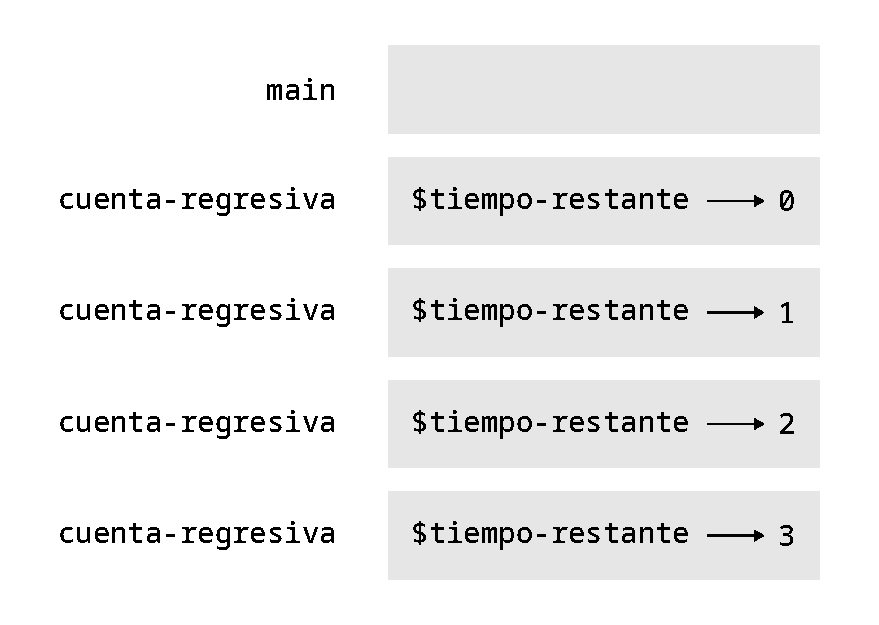
\includegraphics[scale=0.6]{figs/stack2.pdf}}
\caption{Stack diagram.}
\label{fig.stack2}
\end{figure}


Como siempre, la parte superior de la pila es el marco de
del programa principal.

Está vacío porque no creamos ninguna variable dentro del marco.
Tampoco pasamos ningún argumento al marco.
\index{base case}
\index{recursion!base case}

Los cuatro marcos de {\tt cuenta-regresiva} tienen diferente valores
para el parámetro {\tt \$tiempo-restante}. La parte inferior de la 
pila, donde {\tt \$tiempo-restante = 0}, se conoce como el {\bf caso base}.
El caso base no realiza una llamada recursiva y por lo tanto, no hay más
cuadros.

Como ejercicio, dibuja un diagrama de pila para la subrutina \verb|imprime-n-veces|
la cual se llama con los argumentos \verb|$sentence| y {\tt \$n = 2}.
Después escribe una función llamada \verb|hazlo-n-veces| que toma una función
y un número, {\tt \$num}, como argumentos, y llama la función 
provista {\tt \$num} veces.
\label{do_n_times}

Solución: ve la Sección~\ref{sol_do_n_times}


\section{Recursión Infinita}
\index{infinite recursion}
\index{recursion!infinite}
\index{runtime error}


Si una recursión nunca alcanza un caso base, se mantiene 
haciendo llamadas recursivas, y el programa nunca termina. Esto
se conoce como {\bf recursión infinita}, y generalmente no es 
una buena idea. De hecho, tu programa no se ejecutará por siempre
sino que terminará en algún punto cuando la computara agote la 
memoria disponible o algún otro recurso crítico.

Tienes que ser cuidadoso al escribir subrutinas recursivas. 
Asegúrate de tener un caso base, y comprueba que el programa
lo alcanzará. Actualmente, aunque esto no absolutamente requerido
por el lenguaje, te aconsejo que crees el hábito de tratar 
el caso base primero.

\section{Entrada del Teclado}
\index{keyboard input}

Los programas que hemos escrito hasta ahora no aceptan la
entrada de texto por el usuario. Ellos hace la mismas cosas
una y otra vez. Perl provee funciones integradas para parar
el programa y esperar que el usuario escriba algo.

Por ejemplo, la función {\tt prompt} incita al usuario a escribir
algo a través de una pregunta o una instrucción. Cuando el usuario 
presiona {\sf Return} o {\sf Enter}, el programa resume y 
la función \verb|prompt| devuelve lo que el usuario escribió 
como una cadena de texto (sin el carácter de nueva línea que 
corresponde a la tecla {\sf Return} que el usuario pulsa):
\index{prompt function}
\index{function!prompt}

\begin{verbatim}
my $usuario = prompt "Por favor escribe tu nombre: ";
say "Hola $usuario";
\end{verbatim}
%

Esta es probablemente una de las maneras más común de
obtener entrada interactiva de texto por el usuario, porque
es una buena idea dejarle saber lo que se espera.

Otra posibilidad es usar el método {\tt get} (el cual lee
una sola línea) en la entrada estándar:
\index{get function}
\index{function!get}

\begin{verbatim}
say "Por favor escribe tu nombre: ";
my $usuario = $*IN.get;
say "Hola $usuario";
\end{verbatim}
%
o la función {\tt get}, la cual lee una línea de la entrada
estándar por defecto:
\begin{verbatim}
say "Por favor escribe tu nombre: ";
my $usuario = get;
say "Hola $usuario";
\end{verbatim}
%

\section{Argumentos del Programa y la Subrutina MAIN}
\label{MAIN}
\index{MAIN}

Hay otra forma (y usualmente mejor) de hacer que un programa
use entrada variada definida por el usuario, lo cual es 
pasar argumentos desde la línea de comando al programa, de 
la misma manera en la que pasamos argumentos a nuestras subrutinas.

La manera más fácil de extraer argumentos que han sido pasados
al programa es con el uso de la subrutina especial \verb|MAIN|.
Un programa que tiene una subrutina \verb|MAIN| definida
comenzará usualmente su ejecución con esa subrutina, y los argumentos
de la línea de comando suministrados al programa serán pasados
como argumentos a \verb|MAIN|. La signatura \verb|MAIN| te 
permitará extraer los argumentos suministrados en la línea de comando
y posiblemente chequear la validad de los argumentos. 
\index{signature}

Por ejemplo, el programa {\tt saludar.pl6} podría lucir
así:
\begin{verbatim}
sub MAIN (Str $nombre) {
    say "Hola $nombre";
}
\end{verbatim}

Puedes llamar este programa dos veces con diferentes argumentos
en la línea de comando de tal forma:

\begin{verbatim}
$ perl6 saludar.pl6 Larry
Hola Larry

$ perl6 greet.pl6 world
Hola world
\end{verbatim}

Es muy fácil cambiar el argumento, debido a que todo lo que
necesitas hacer en la línea de comando del sistema operativo
es usar la flecha y editar el final de la línea de comando
anterior.

Si olvidas suministrar un argumento (o provees el número 
equivocado de argumentos, o los argumentos no coinciden con
la signatura), el programa terminará y Perl~6 generará
y mostrará el modo de uso:

\begin{verbatim}
$ perl6 saludar.pl6
Usage:
  saludar.pl6 <nombre>
\end{verbatim}


\section{Depuración de programas}
\label{whitespace}
\index{debugging}
\index{traceback}

Cuando ocurre un error de sintaxis o un error al tiempo de ejecución,
el mensaje de error contiene mucha información, aunque puede ser
agobiante. Las preguntas más útiles son usualmente:

\begin{itemize}

\item ¿Qué tipo de error fue?

\item ¿Dónde ocurrió?

\end{itemize}

Los errores sintácticos son usualmente fáciles de encontrar,
sin embargos existen algunos trucos. En general, los mensajes 
de error indican donde se descubrió el problema, aunque el actual
error podría encontrarse un poco antes, algunas veces en la 
línea previa o hasta varias líneas antes.
\index{multiplication tables}

Por ejemplo, el objetivo del siguiente código era mostrar
la tabla de multiplicación:

\begin{verbatim}
# ADVERTENCIA: código con fallas
sub tabla-multiplicación {
    for 1..10 -> $x {
        for 1..10 -> $y {
            say "$x x $y\t= ", $x * $y;
        say "";
    }
}

tabla-multiplicación();
\end{verbatim}

Falló al tiempo de compilación con el siguiente error:

\begin{verbatim}
$ perl6 tabla_mult.pl6
===SORRY!=== Error while compiling /home/Laurent/tabla_mult.pl6
Missing block (taken by some undeclared routine?)
at /home/Laurent/tabla_mult.pl6:9
------> tabla-multiplicación();<HERE><EOL>
\end{verbatim}

El mensaje de error reporta un error en la línea~9 del 
programa (la última línea del código), al final de la línea,
pero el error actual es que falta una llave izquierda después
de la línea~4 y antes de la línea~5. La razón de esto es que,
mientras el programador cometió el error en la línea~4,
el interpretador de Perl no pudo detectar este error antes 
de alcanzar el final del programa. El programa correcto para mostrar
la table de multiplicación podría ser:

\begin{verbatim}
sub tabla-multiplicación {
    for 1..10 -> $x {
        for 1..10 -> $y {
            say "$x x $y\t= ", $x * $y;
        }
        say "";
    }
}
tabla-multiplicación();
\end{verbatim}

Cuando un error es reportado en la última línea de un
programa, es comúnmente causado por la falta de un
paréntesis, un corchete, una llave, o una comilla varias
líneas más arriba. Un editor con coloración de sintaxis
puede algunas veces ayudarte a resolver este error.
\index{syntax!highlighting}

\index{error!runtime}
\index{runtime error}

Lo mismo sucede con errores al tiempo de ejecución. Considera
este programa cuyo objetivo es calcular 360 grados divididos
sucesivamente por los enteros entre 2 y 5:

\begin{verbatim}
# ADVERTENCIA: código con fallas
my ($a, $b, $c, $d) = 2, 3, 5;
my $valor = 360;
$valor /= $_ for $a, $b, $c, $d;
say $valor;
\end{verbatim}

Esto programa compila correctamente pero muestra una
advertencia y después una excepción al tiempo de ejecución:

\begin{verbatim}
Use of uninitialized value of type Any in numeric context 
in block  at producto.pl6 line 3
Attempt to divide 12 by zero using div
  in block <unit> at producto.pl6 line 4
\end{verbatim}
%

El mensaje de error indica una excepción ``division by zero''
en la línea~4, pero no hay nada
incorrecto con esa línea. La advertencia en la línea~3
podría darnos una pista sobre el intento del script 
de usar un valor indefinido, pero el error real se encuentra 
en la primera línea del script, donde uno de los cuatros 
enteros necesarios fue omitido por equivocación en la
asignación de la lista.

\index{division by zero}
\index{uninitialized value}

Deberías prestarle atención a los mensajes de error y leerlos
cuidadosamente. Sin embargo, no asumas que ellos apuntan a la
causa de la excepción; usualmente ellos apuntan 
a problemas subsecuentes.


\section{Glosario}

\begin{description}

\item[División de enteros] Una operación, denotada por {\tt div},
que divide dos números y redondea el resultado.
  \index{integer division} 
  \index{division!integer}

\item[Operador de módulo]  Un operador, denotado por un signo
de porcentaje ({\tt \%}), que funciona con números enteros y devuelve
el residuo al dividir un número por otro.
\index{modulo operator}
\index{operator!modulo}

\item[Expresión Booleana]  Una expresión cuyo valor es 
{\tt True} o {\tt False}.
\index{Boolean expression}
\index{expression!Boolean}

\item[Operador de relación] Uno de los operadores que compara
sus operandos. Los operadores de relación numérica más comunes son 
{\tt ==}, {\tt !=}, {\tt >}, {\tt <}, {\tt >=}, y {\tt <=}. 
Los operadores equivalentes de relación de cadenas de texto 
son {\tt eq}, {\tt ne}, {\tt gt}, {\tt lt}, {\tt ge}, and {\tt le}.

\item[Operador lógico] Uno de los operadores que combina expresiones
Booleanas: {\tt and}, {\tt or}, y {\tt not}. Los 
operadores equivalentes de precedencia superior son
{\tt \&\&}, {\tt ||}, y {\tt !}

\item[Sentencia condicional]  Una sentencia que controla el flujo
de ejecución dependiendo en algunas condiciones.
\index{conditional!statement}
\index{statement!conditional}

\item[Condición] La expresión booleana en una sentencia
condicional que determina cual de las ramas se ejecuta.
\index{condition}

\item[Rama] Una de las secuencias alternativas de sentencias
en una sentencia condicional.
\index{branch}

\item[Condicional encadenada]  Una sentencia condicional con 
una serie de ramas alternativas.
\index{chained conditional}
\index{conditional!chained}

\item[Condicional anidada]  Una sentencia condicional que aparece
en una de las ramas de otra sentencia condicional.
\index{nested conditional}
\index{conditional!nested}

\item[Modificador de sentencia] Una expresión condicional sufija,
i.e., una expresión condicional (usando por ejemplo {\tt if}, {\tt unless} o 
{\tt for}) que es colocada después de la sentencia cuya ejecución
controla. También puede referirse a una expresión de bucle sufijo.
\index{statement modifier}

\item[Sentencia de retorno] Una sentencia que forza a una 
función a terminar de inmediato y devolver a la función
que realiza la llamada.

\item[Recursión]  El proceso de llamar una función 
que aún está en ejecución.
\index{recursion}

\item[Caso base]  Una rama condicional en una función
recursiva que no realiza una llamada recursiva.
\index{base case}

\item[Recursión infinita]  Una recursión que carece
de un caso base, o que nunca lo alcanza. Eventualmente, 
una recursión infinita causa un error al tiempo de ejecución,
por el cual no querrás esperar dado que podría tardar demasiado.
\index{infinite recursion}

\end{description}

\section{Ejercicios}
%

\begin{exercise}
%
Usando los operadores división de enteros y módulo:
\index{modulo operator}
\index{operator!mod}
\index{mod, modulo operator}
\index{integer division}
\index{operator!div}
\index{div operator}
\label{int_div_modulo}

\begin{enumerate}

\item Escribe una subrutina que calcule cuantos días, horas, minutos y segundos
hay en el número de segundos pasado como argumento a la subrutina.

\item Escribe un script que calcule cuantos días, horas, minutos y segundos 
hay en 240, 000 segundos.

\item Cambia el script para calcular el número de días, horas, minutos y segundos
que hay en un número de segundos proveído por el usuario cuando se le
pide proveer un número de segundos.

\end{enumerate}

Soluciones: Subsección~\ref{sol_int_div_modulo}.

\end{exercise}


\begin{exercise}
\index{Fermat's Last Theorem}
\label{fermat_ex}

El último teorema de Fermat enuncia que no existen números enteros
positivos $a$, $b$, y $c$ tales que se cumpla:

\[ a^n + b^n = c^n \]
%
para todos los valores de $n$ mayores que 2.

\begin{enumerate}

\item Escribe una función con el nombre \verb|chequear-fermat| que
toma cuatro parámetros---{\tt a}, {\tt b}, {\tt c}, y {\tt n}---y
chequea si se cumple el teorema de Fermat. Si $n$ es mayor que 2 y 

\[a^n + b^n = c^n \]
%
el programa debería imprimir, ``¡Santo dios, Fermat estaba equivocado!``
Por lo contrario, el programa debería imprimir ``Ǹo, eso no funciona.``

\item Escribe una subrutina que incita al usuario a entrar valores para 
las variables {\tt a}, {\tt b}, {\tt c}, y {\tt n}, los convierte a enteros,
y usa la función \verb|chequear-fermat| para chequear si ellos violan
el teorema de Fermat.
\end{enumerate}

Solución: \ref{sol_fermat_ex}


\end{exercise}


\begin{exercise}
\index{triangle}
\label{triangle}

Si se te provee con tres palillos, podrías o no podrías 
ser capaz de organizarlos en un triángulo.
Por ejemplo, si uno de los palillos tiene una longitud de 
12 pulgadas y los restantes tienen 1 pulgada, no podrás
conseguir que los palillos pequeños se encuentren en 
el medio. Para tres longitudes cualquiera, existe una 
simple prueba para ver si es posible crear un triángulo:

\begin{quotation}
Si una de las tres longitudes es mayor que la suma de las
otras dos, entonces no puedes formar una triángulo. De lo
contrario, puedes formar un triángulo. (Si la suma de dos
lados es igual al tercero, ellos forman lo que se
conoce como un triángulo "degenerado".)
\end{quotation}

\begin{enumerate}

\item Escribe una función llamada \verb|es-triángulo| que toma
tres números positivos como argumentos, e imprime ``Sí`` o ``No,``
dependiendo si puedes formar un triángulo con las longitudes
dadas.

\item Escribe una función que incite al usuario a entrar
tres longitudes y use la función \verb|es-triángulo| para 
chequear si palillos con las longitudes dadas pueden formar 
un triángulo.
\end{enumerate}

Solución: \ref{sol_triangle}


\end{exercise}

\begin{exercise} 
\index{Fibonacci!numbers}
\label{fibonacci}
Los números Fibonacci fueron inventados por Leonardo Fibonacci 
(también conocido como Leonardo de Pisa o simplemente, Fibonacci), 
un matemático italiano del siglo XIII.
\index{Fibonacci, Leonardo}

Los números Fibonacci son una secuencia de números como tal:

\[1, \;1, \;2, \;3, \;5, \;8, \;13, \;21, \;34, \ldots\]
%
en la cual los primeros dos números son 1 y cada número 
subsecuente de la secuencia está definido como la suma de
los dos números anteriores (por ejemplo, $5 = 2 + 3$, $8 = 3 + 5$, etc.).

En notación matemática, los números Fibonacci 
podrían ser definidos por una relación de recurrencia  
de la siguiente manera:

\[F_1 = 1, \;F_2 = 1, \;\;and\;\;  F_n = F_{n-1} + F_{n-2} \]
%
\begin{enumerate}

\item  Escribe un programa usando el bucle {\t for} que imprime
en la pantalla los primeros 20 números Fibonacci.

\item Escribe un programa que incite al usuario a entrar un número $n$ y,
usando el bucle {\tt for}, calcule y muestre el número Fibonacci $n^{th}$.
\end{enumerate}

Solución: \ref{sol_fibonacci}


\end{exercise}

\begin{exercise}
\label{sub_recurse}
\index{recursion}

¿Cuál es la salida del siguiente programa?
Dibuja un diagrama de pila que muestre el estado del 
programa cuando imprime el resultado.

\begin{verbatim}[fontshape=up]
sub recurse($n, $s) {
    if ($n == 0) {
        say $s;
    } else {
        recurse $n - 1, $n + $s;
    }
}
recurse 3, 0;
\end{verbatim}

\begin{enumerate}

\item ¿Qué pasaría si llamaras la función de la siguiente forma:
{\tt recurse(-1, 0)}?

\item Escribe un comentario de documentación (quizás en la forma de un comentario multilínea) que explique todo lo que alguien necesita saber para usar esta función (y nada más).
\end{enumerate}

Solución: \ref{sol_sub_recurse}

\end{exercise}


